\section{Auswertung}
\label{sec:Auswertung}

\subsection{Amplitudenmodulierte Schwingung mit Ringmodulator}

Mit Hilfe der Schaltung aus Abbildung \ref{fig:???} wird eine Amplitudenmodulierte Schwingung erzeugt.
Diese so entstandene Schwebung ist in Abbildung \ref{fig:amplModOszi} zu sehen.

\begin{figure}[H]
  \centering
  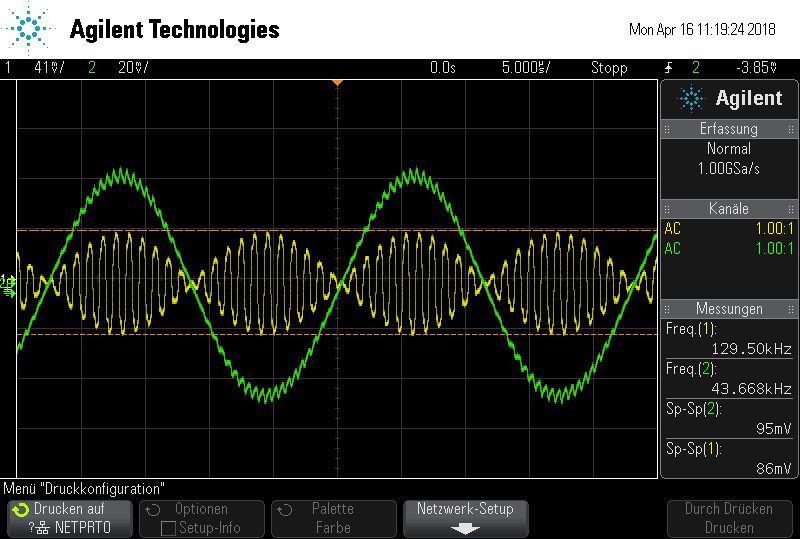
\includegraphics[width=\textwidth]{Oszi_Pics/amplModRing.png}
  \caption{Amplitudenmodulierte Schwingung(gelb) und Modulationsschwingung(grün) erzeugt mit Ringmodulator.}
  \label{fig:amplModOszi}
\end{figure}

Die mit dem Oszilloskop außerdem ausgemessenen Werte für die Frequenzen $\omega$ und Amplituden $U_\text{peak to peak}$ der Modulationsspannung $M$ und der Trägerspannung $T$ sind:

\begin{align*}
  \omega_\text{M} &= \SI{43.8(5)}{\kilo\hertz} & U_\text{M, ptp} &= \SI{95(1)}{\milli\volt}\\
  \omega_\text{T} &= \SI{970(1)}{\kilo\hertz} & U_\text{T, ptp} &= \SI{540(1)}{\milli\volt}.
\end{align*}

Die mit dem Frequenzspektrometer aufgenommenen Werte sind in den Bildern \ref{fig:b1}, \ref{fig:b2} und \ref{fig:b3} zu sehen.

\begin{figure}[H]
  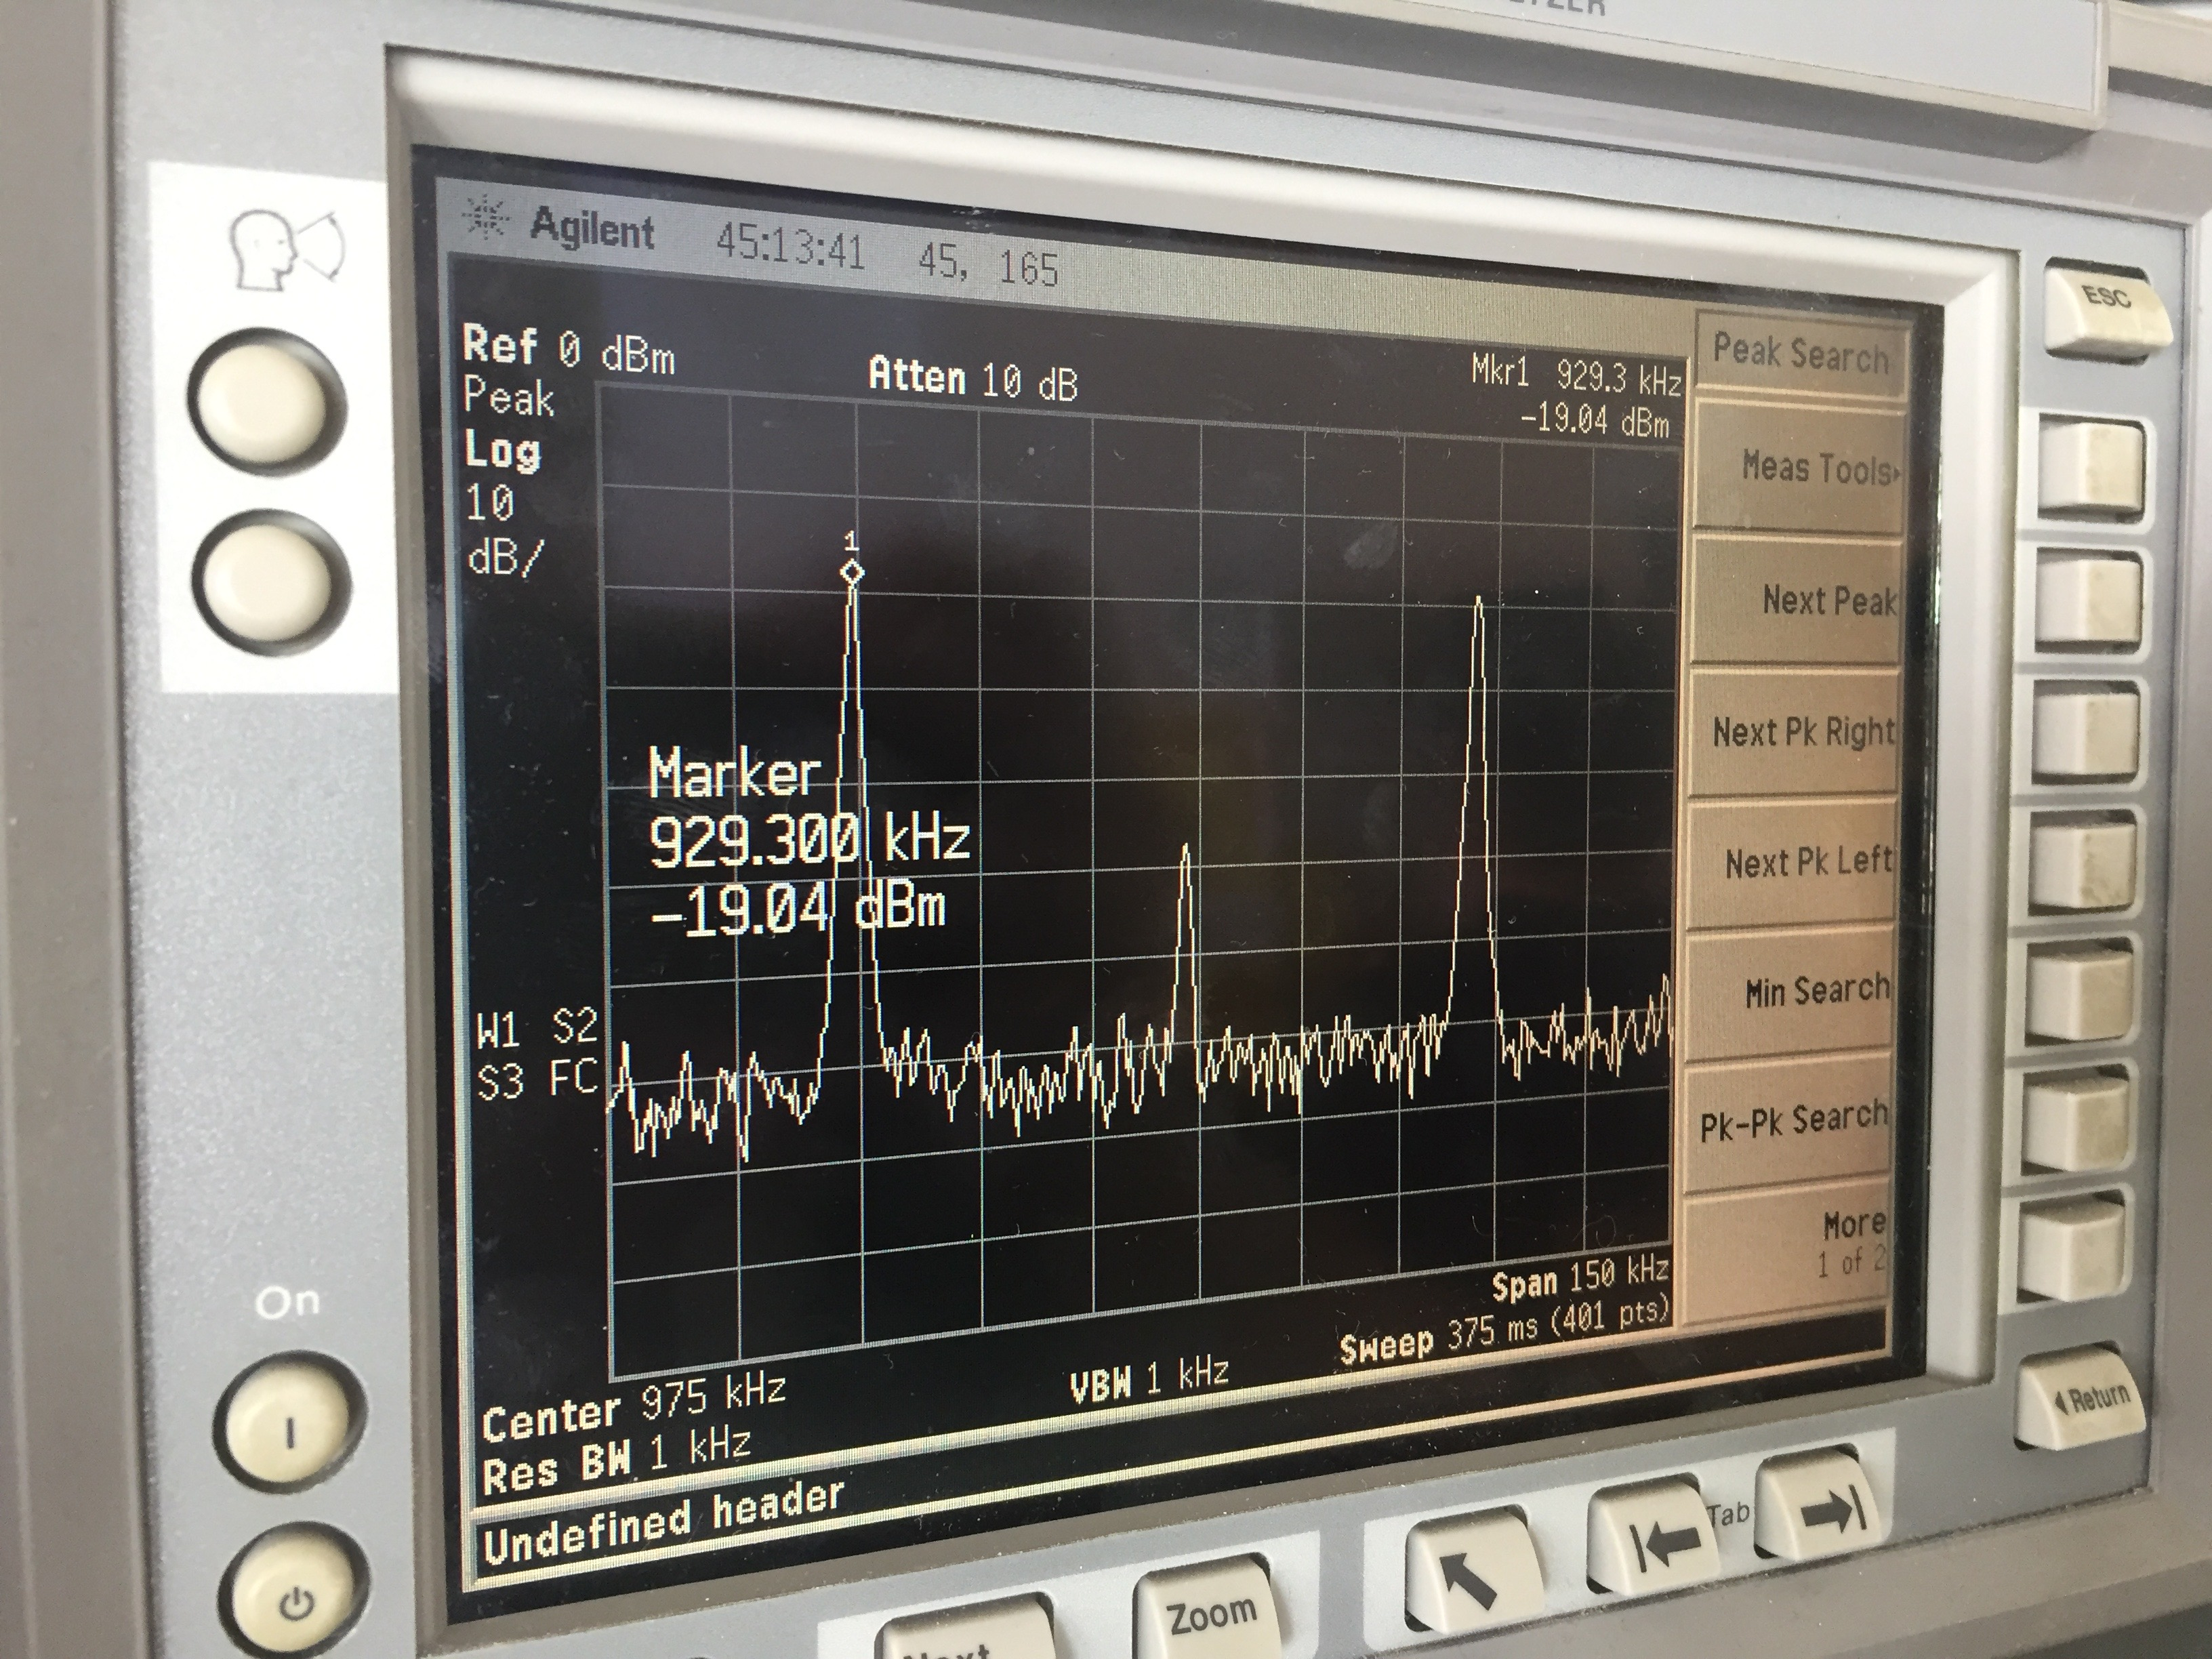
\includegraphics[width=\textwidth]{Spektrum_Pics/b1.jpg}
  \caption{Spektrum der mit dem Ringmodulator amplitudenmodulierten Schwingung mit Markierung vom Peak $\omega_\text{T} - \omega_\text{M}$}
  \label{fig:b1}
\end{figure}
\begin{figure}[H]
  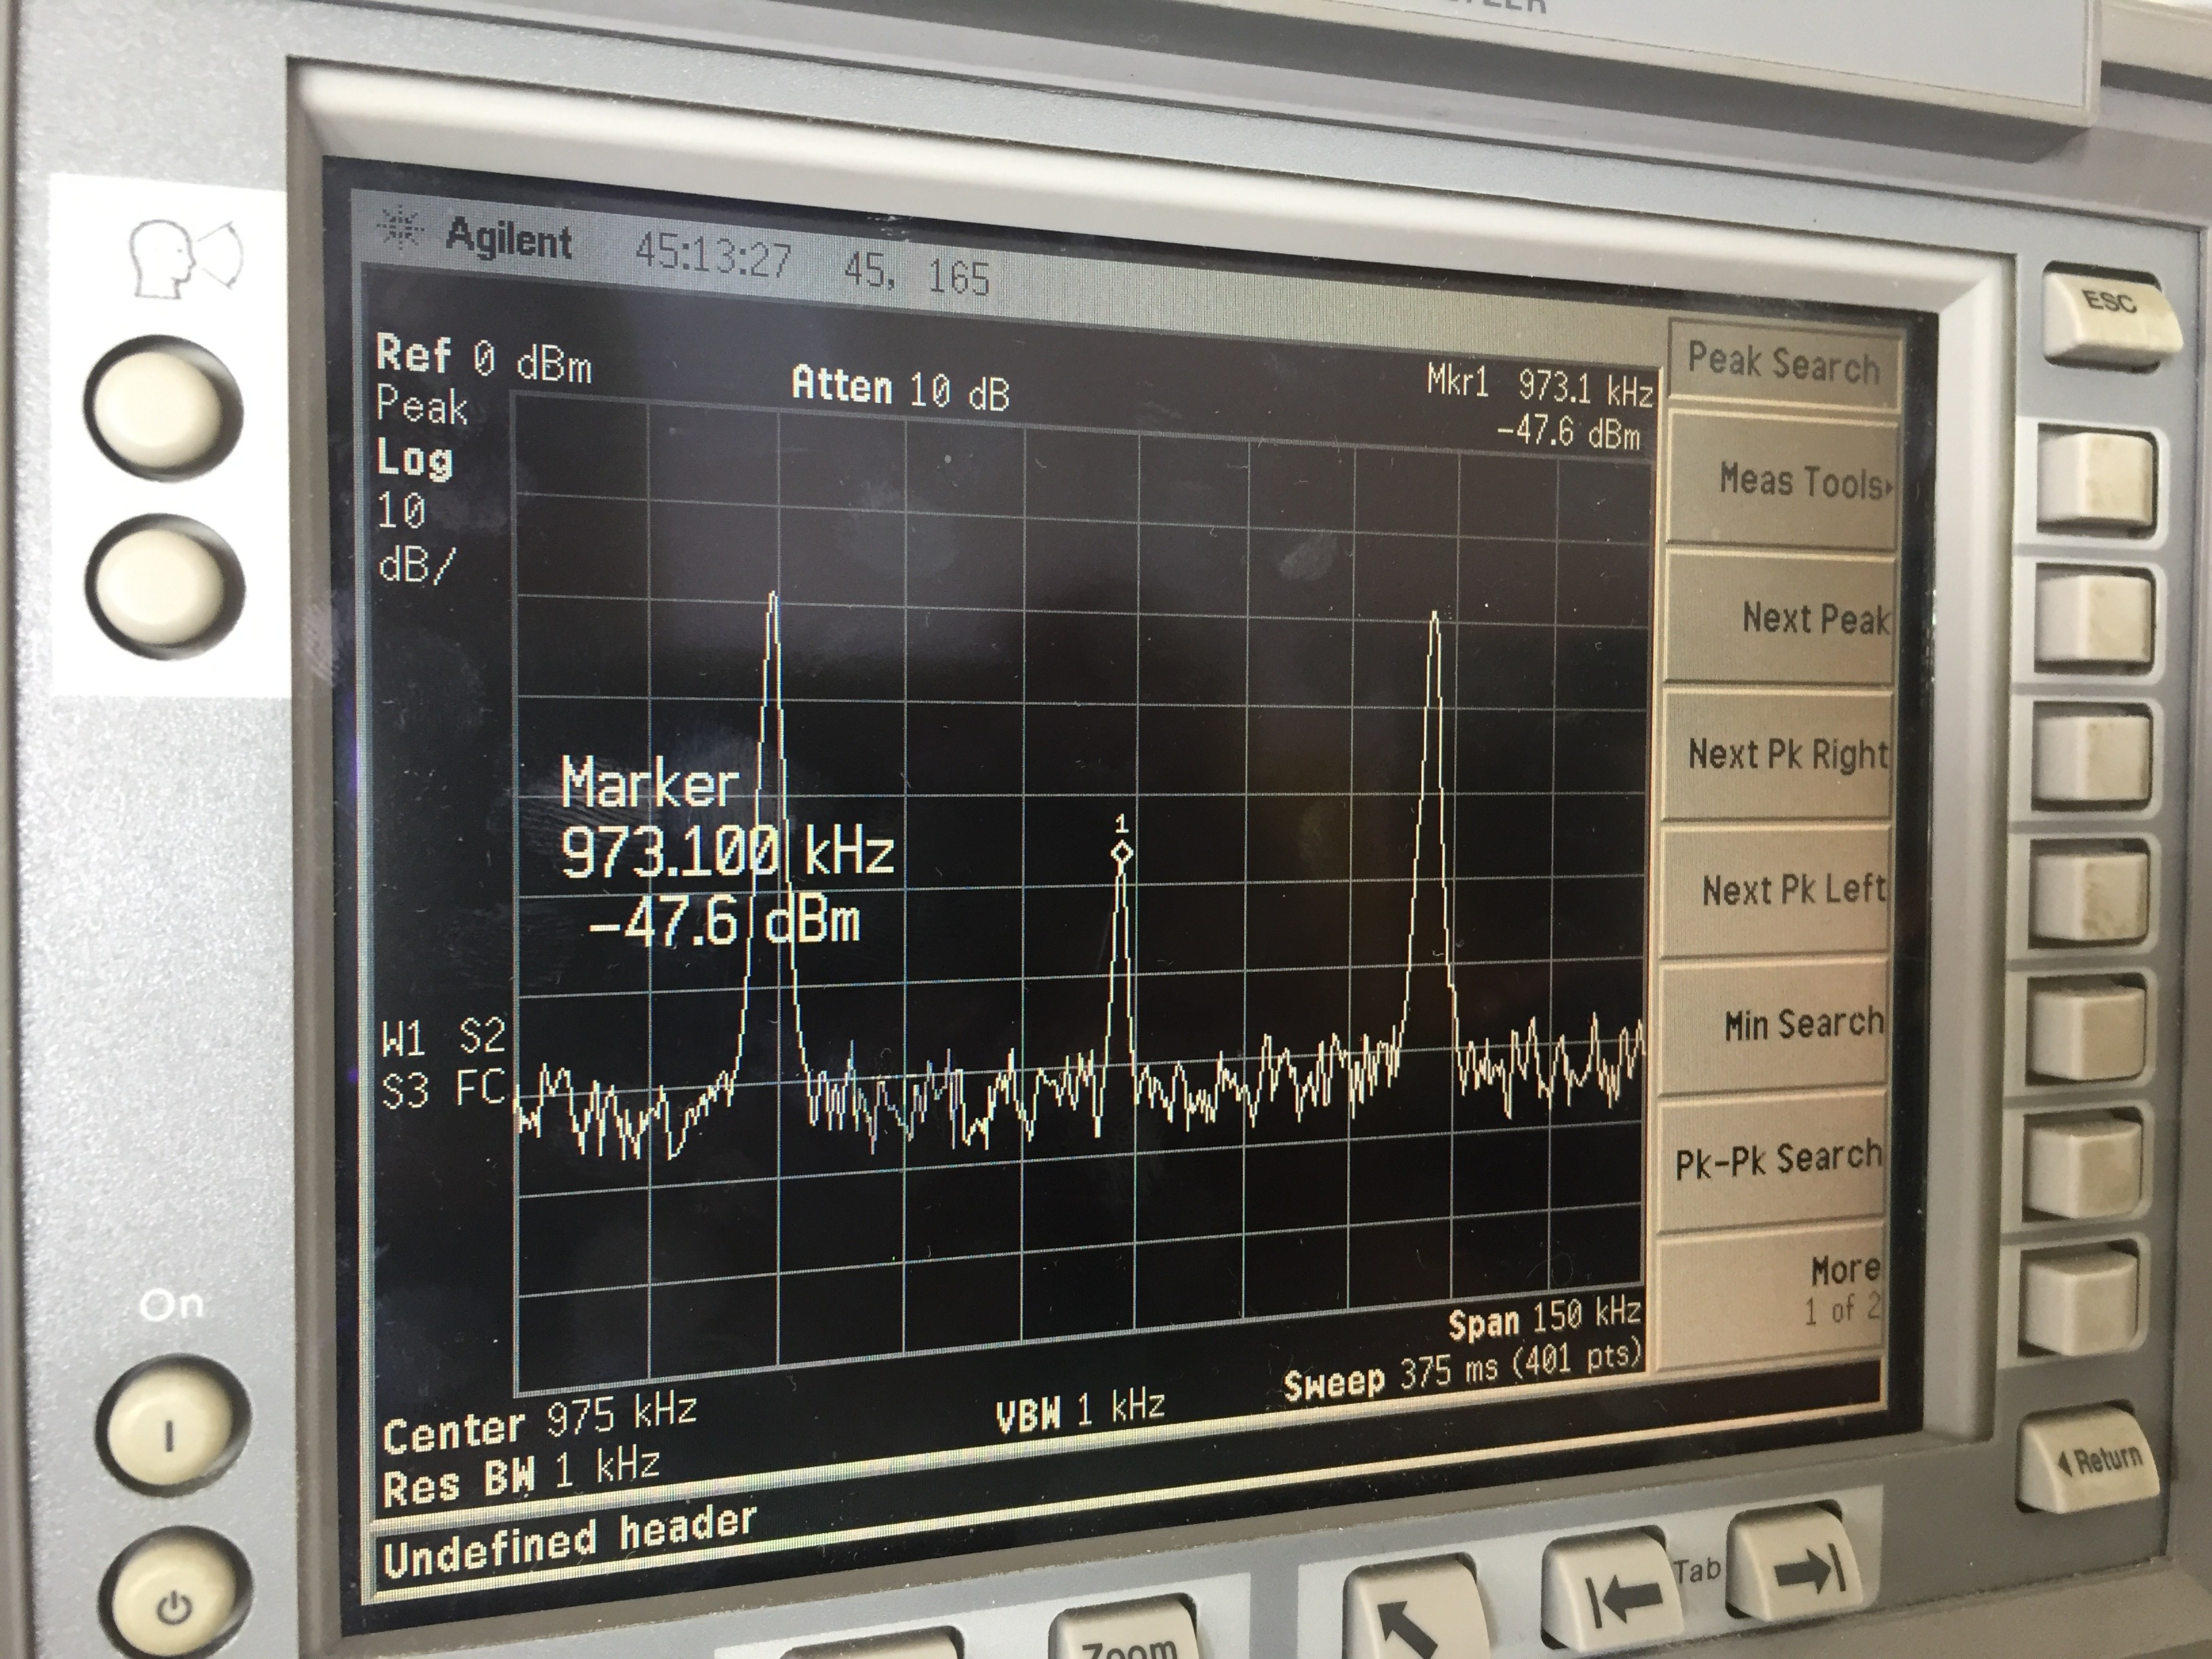
\includegraphics[width=\textwidth]{Spektrum_Pics/b2.jpg}
  \caption{Spektrum der mit dem Ringmodulator amplitudenmodulierten Schwingung mit Markierung vom Peak $\omega_\text{T}$}
  \label{fig:b2}
\end{figure}
\begin{figure}[H]
  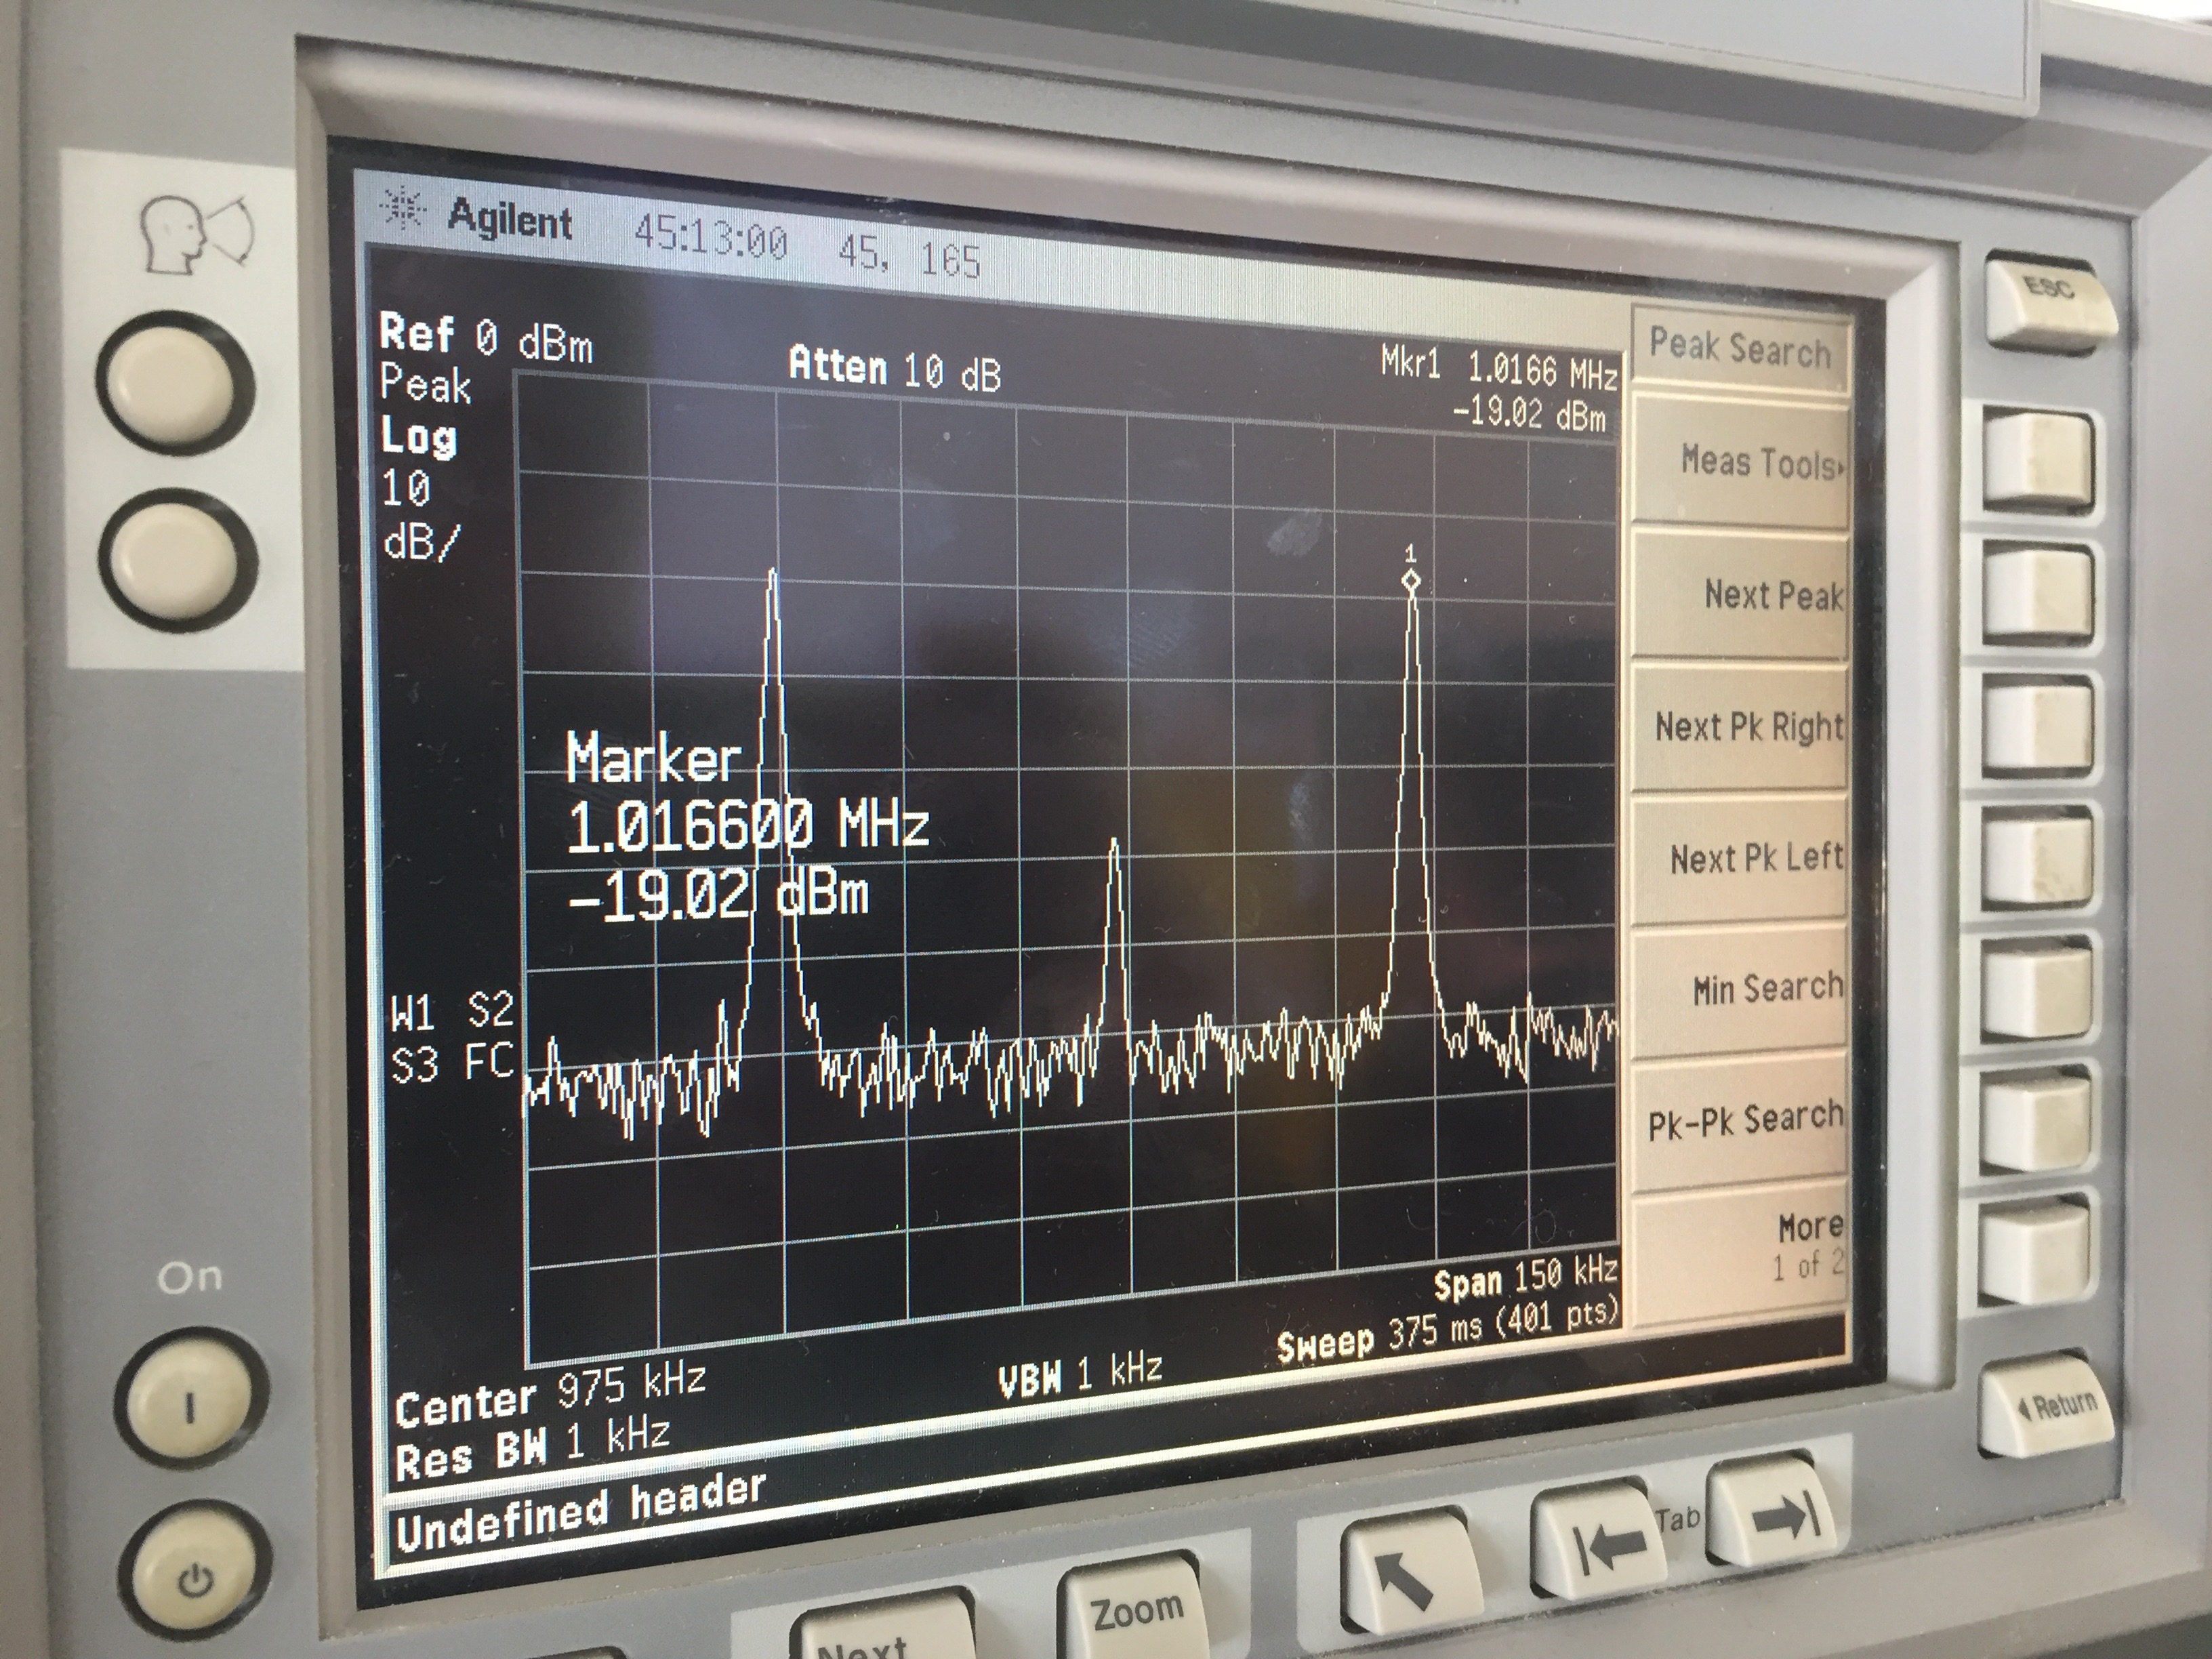
\includegraphics[width=\textwidth]{Spektrum_Pics/b3.jpg}
  \caption{Spektrum der mit dem Ringmodulator amplitudenmodulierten Schwingung mit Markierung vom Peak $\omega_\text{T} + \omega_\text{M}$}
  \label{fig:b3}
\end{figure}

Die aus dem Frequenzspektrum abgelesenen Frequenzen für die drei größten Peaks sind:
\begin{align*}
  \omega_1 &= \SI{929.3}{\kilo\hertz} & \omega_2 &= \SI{973.1}{\kilo\hertz} & \omega_3 &= \SI{1016.6}{\kilo\hertz}.\\
\end{align*}
Die Abweichungen zu den erwarteten Werten betragen:
\begin{align*}
  \frac{|(\omega_\text{T} - \omega_\text{M}) - \omega_1|}{\omega_\text{T} - \omega_\text{M}} &= \SI{0.3(1)}{\percent}\\
  \frac{|\omega_\text{T} - \omega_2|}{\omega_\text{T}} &= \SI{0.3(1)}{\percent}\\
  \frac{|(\omega_\text{T} + \omega_\text{M}) - \omega_3|}{\omega_\text{T} + \omega_\text{M}} &= \SI{0.3(1)}{\percent}.
\end{align*}

\subsection{Amplitudenmodulierte Schwingung mit Diode}

Nach Schaltung aus Abbildung \ref{fig:???} wird hier der allgemeine Fall der Amplitudenodulation mit einer Diode gezeigt.

\begin{figure}[H]
  \centering
  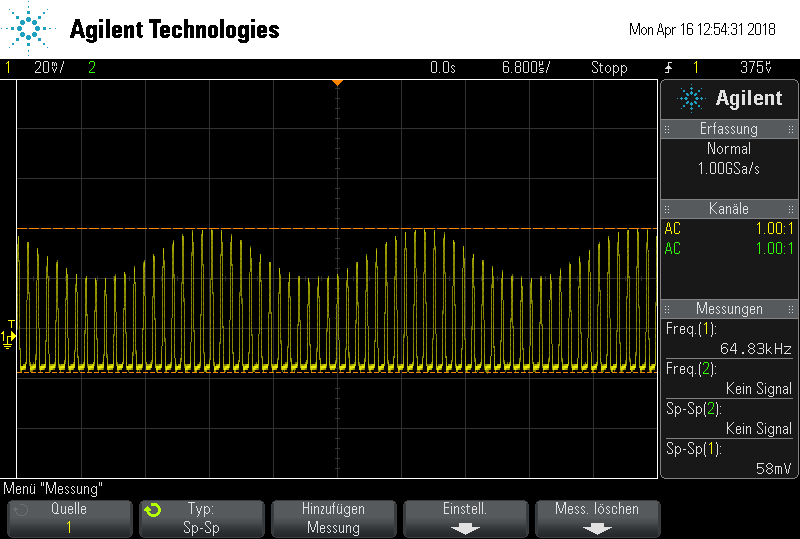
\includegraphics[width=\textwidth]{Oszi_Pics/amplModDiode.png}
  \caption{Amplitudenmodulierte Schwingung erzeugt mit einer Diode.}
  \label{fig:amplModDiode}
\end{figure}

Die so entstandene Schwebung ist in Abbildung \ref{fig:amplModDiode} zu sehen.
Außerdem wurden folgende Kenzahlen der modulierten Spannung ausgemessenen:
die Spannungsdifferenz von der Nulllinie im Oszilloskop bis zum höchsten Wert $U_\text{T, max}$, die Differenz zwischen der höchsten und der niedrigsten Amplitude $U_\text{diff}$ sowie die Spannungsdifferenz von der Nulllinie bis zur unteren Kante also der Fehler der Diode $U_\text{fehler}$.
Diese Werte betragen:
\begin{align*}
  U_\text{T, max} &= \SI{43.25(2)}{\milli\volt} & U_\text{diff} &= \SI{19.75(2)}{\milli\volt}  & U_\text{fehler} &= \SI{13.75(2)}{\milli\volt}
\end{align*}
Aus Bild \ref{fig:???} wird die Formel
\begin{align}
  m &= \frac{U_\text{T, max}}{U_{\hat T}}\\
  \intertext{hergeleitet; mit}
  U_{\hat T} &= U_\text{T, max} - \frac{U_\text{diff}}{2}.
  \intertext{Das ergibt für den Modulationsgrad:}
  m &= \num{0.2959(4)}.
\end{align}

Nun wird der Modulationsgrad aus der Frequenzspektrumsmessung abgelesenen.

\begin{figure}[H]
  \centering
  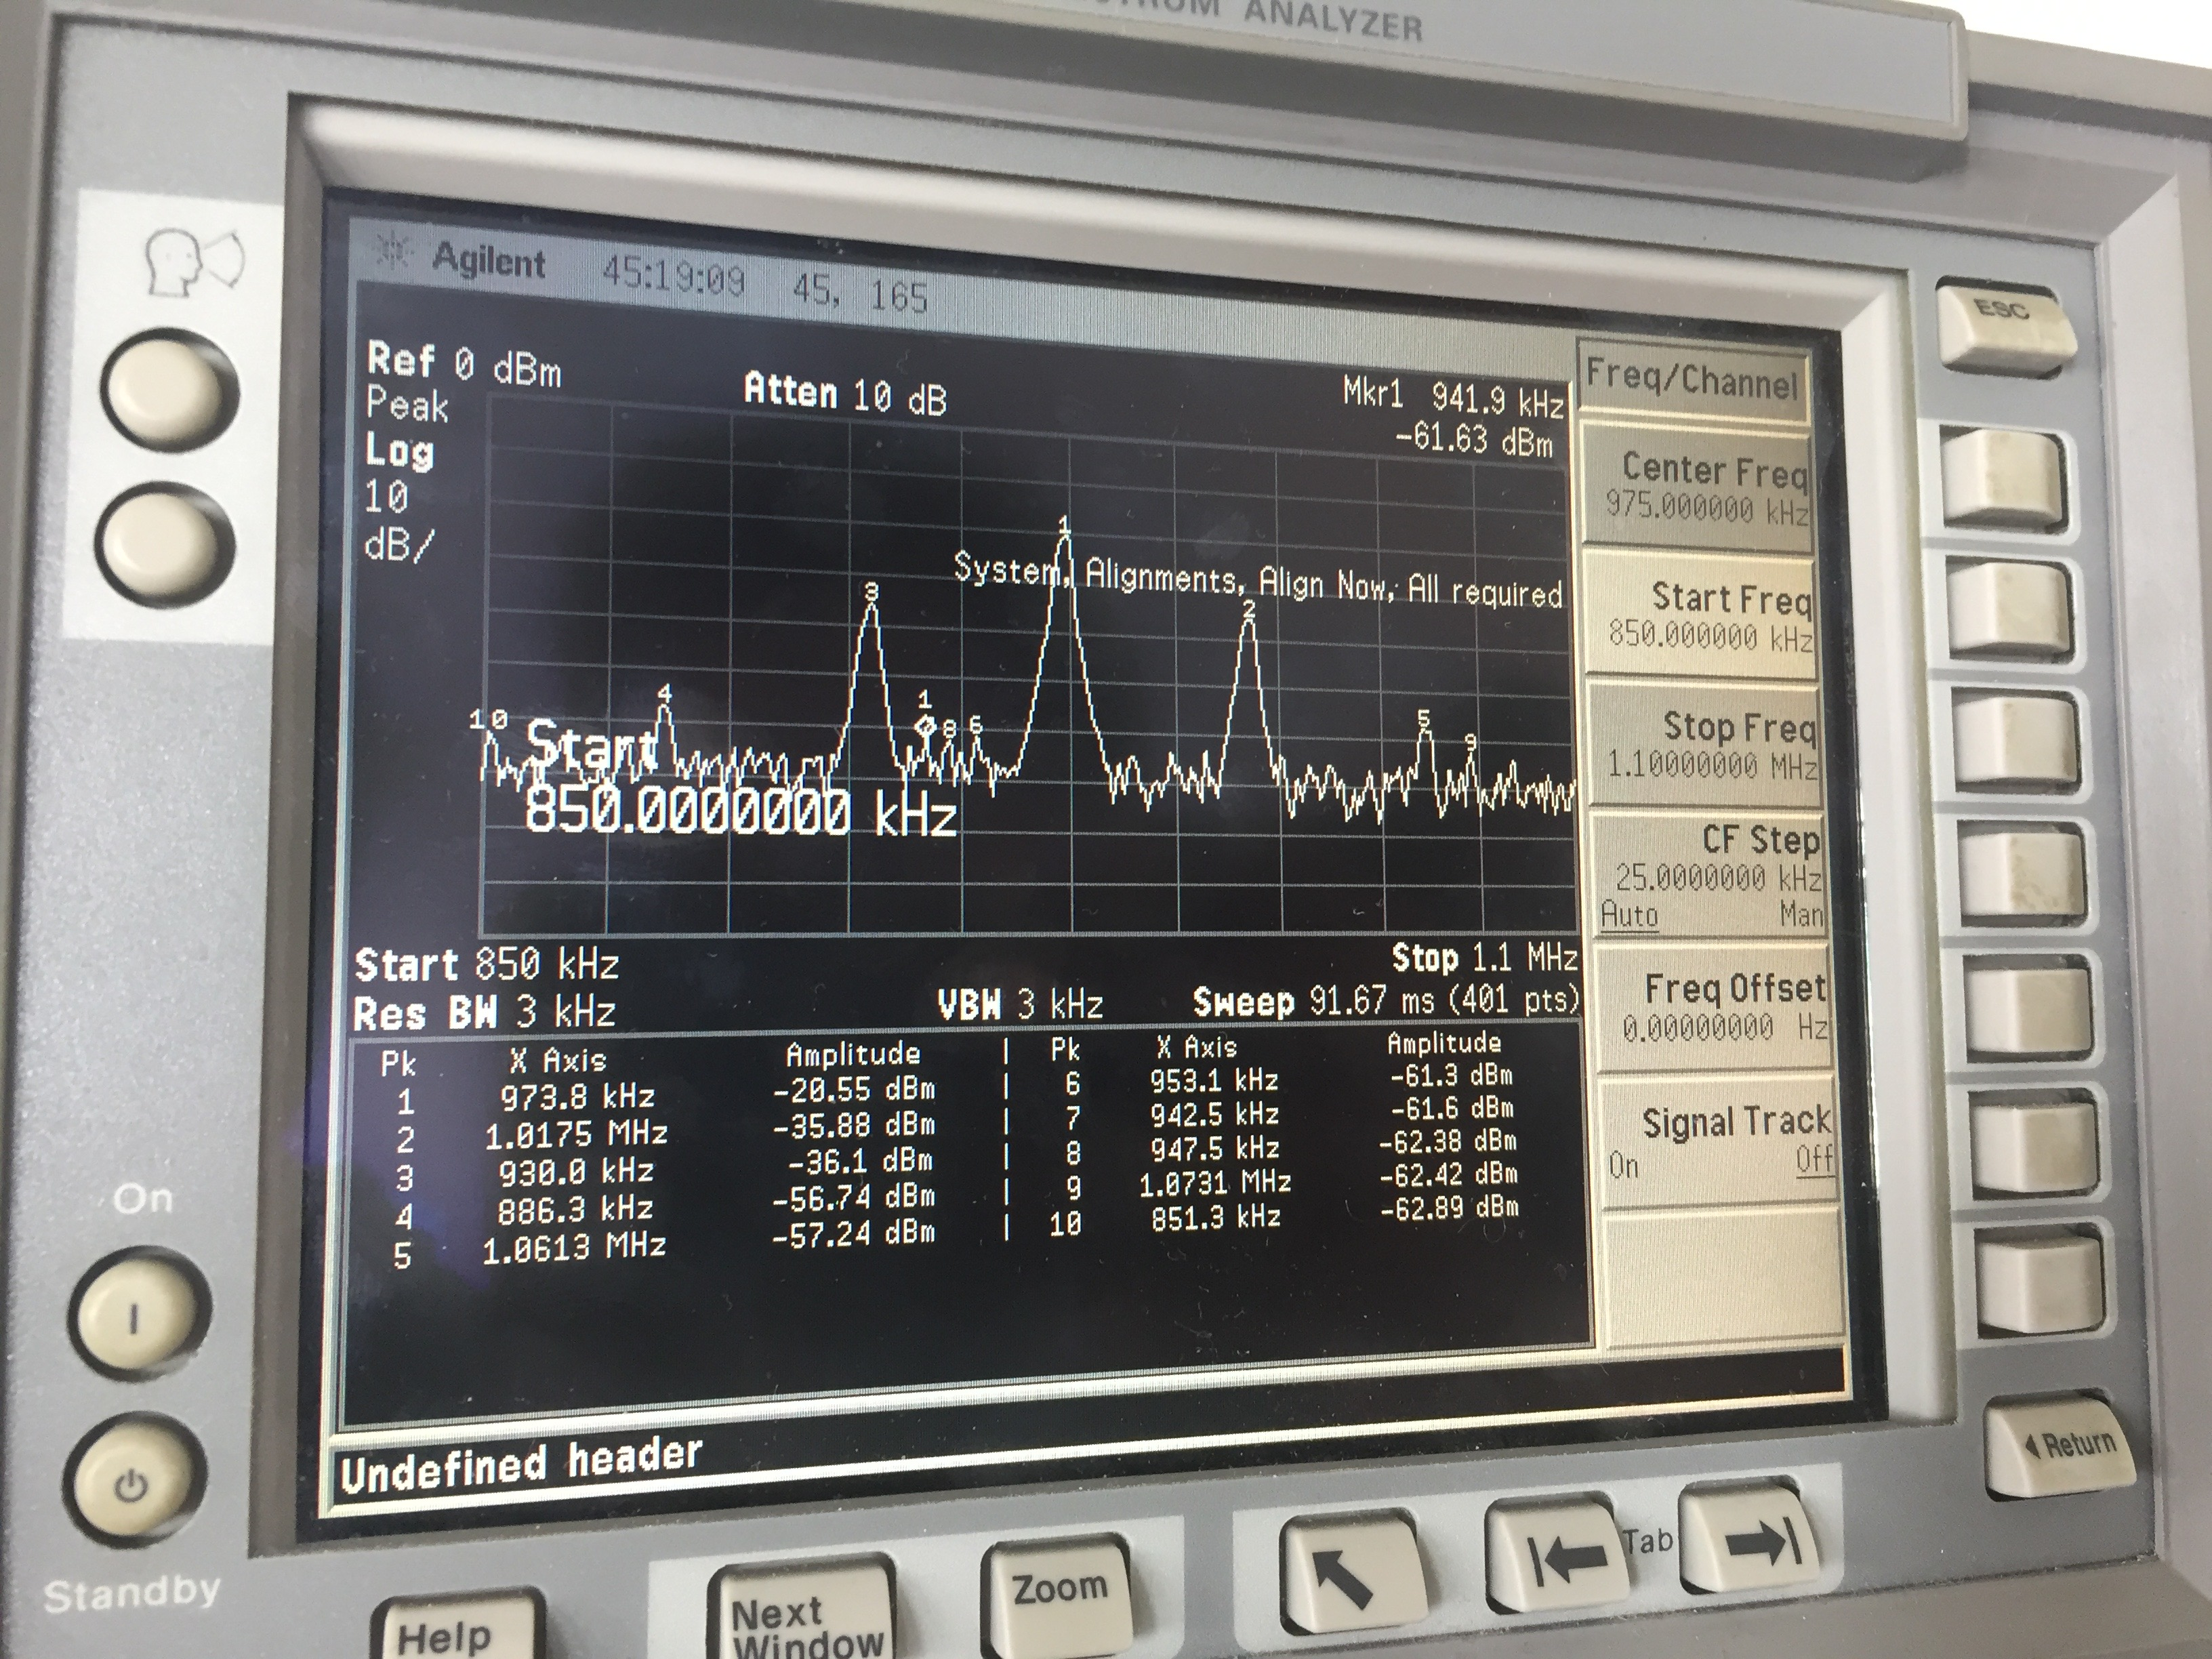
\includegraphics[width=\textwidth]{Spektrum_Pics/c.jpg}
  \caption{Spektrum der mit der Diode amplitudenmodulierten Schwingung mit einer Peaktable.}
  \label{fig:c}
\end{figure}

Das Bild mit dem Spektrum der Frequenzen ist in Abbildung \ref{fig:c} zu sehen.
Dabei werden die drei höchsten Peaks den Frequenzen $\omega_\text{T} - \omega_\text{M}$, $\omega_\text{T}$ und $\omega_\text{T} + \omega_\text{M}$ zugeordnet.
Die abgelesenen Werten für die Leistungspegel $L_\text{P}$ werden nun mit Gleichung \eqref{eqn:dBmTomW} aus \cite{leistungspegel} umgerechnet in Werte für die Leistung der Frequenzen.
\begin{align}
  P(\si{\milli\watt}) =
   10^{\frac{L_\text{P}(\si{dBm})}{10}} \SI{1}{\milli\watt} \label{eqn:dBmTomW}
\end{align}

Diese betragen:
\begin{align*}
  P_\text{links} &= \SI{0.246(1)}{\micro\watt} & P_\text{mitte} &= \SI{8.81(4)}{\micro\watt} & P_\text{rechts} &= \SI{0.258(1)}{\micro\watt}.
\end{align*}

Aus Bild \ref{fig:???} wird nun die Formel zur Bestimmung des Modulationsgrad aus einem Frequenzspektrum hergeleitet:
\begin{align*}
  m &= \frac{2 P_\text{lr}}{P_\text{mitte}}.
\end{align*}

Hierbei ist $P_\text{lr}$ der Mittelwert des linken und des rechten Peaks der drei Peaks mit der höchsten Leistung. Hier wird genutzt, dass $P \propto U$ und so die Leistungen eingesetzt, da ja ein Verhältnis bestimmt wird.
So ergibt sich für $m$:
\begin{align*}
  m &= \num{0.0572(3)}.
\end{align*}

\subsection{Frequenzmodulierte Schwingung}

\begin{figure}[H]
  \centering
  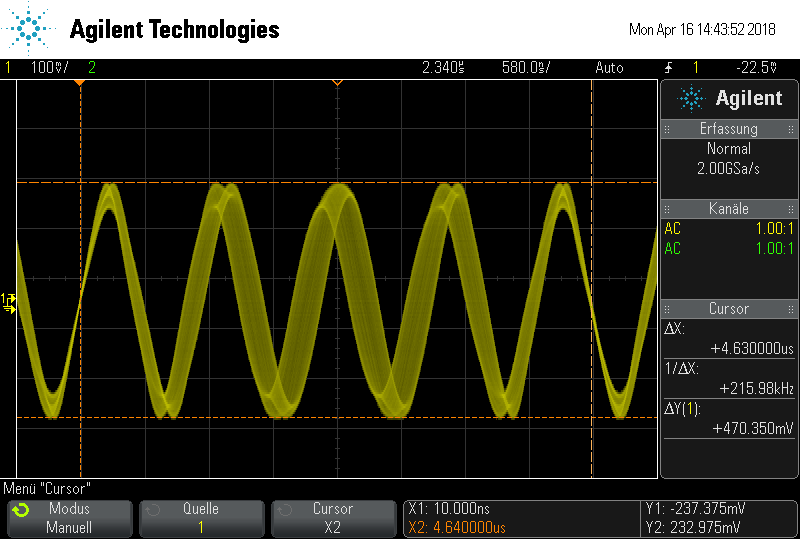
\includegraphics[width=\textwidth]{Oszi_Pics/freqModRing.png}
  \caption{Oszilloskopbild der frequenzmodulierten Schwingung.}
  \label{fig:freqModRing}
\end{figure}

\begin{figure}[H]
  \centering
  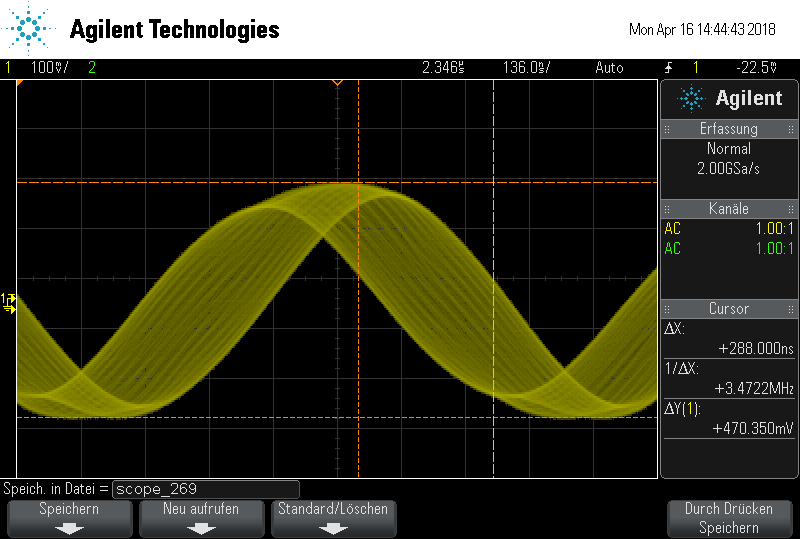
\includegraphics[width=\textwidth]{Oszi_Pics/freqModZoom.png}
  \caption{Vergrößertes Oszilloskopbild der frequenzmodulierten Schwingung.}
  \label{fig:freqModZoom}
\end{figure}

In Abbildung \ref{fig:freqModRing} ist die in X-Richtung verschmierte Sinuskurve der nach Schaltung \ref{fig:???} frequenzmodulierten Schwingung zu sehen. Außerdem ist in Abbildung \ref{fig:freqModZoom} eine vergrößerte Version der Schwingung zu sehen. Daraus wird die Zeitdifferenz bei maximaler Frequenzvariation abgelesenen:
\begin{align*}
  t_2 - t_1 &= \SI{288(5)}{\nano\second}.\\
\intertext{Mit der Kenntnis der Modulationsfrequenz}
  \omega_\text{M} &= \SI{211.5(4)}{\kilo\hertz}\\
\intertext{ergibt sich eingesetzt in Formel \eqref{eqn:???} für den Modulationsgrad}
  m &= \num{0.0416(7)}.
\end{align*}


\subsection{Demodulation mithilfe eines Ringmodulators}

Mit der Schaltung aus Abbildung \ref{fig:???} wird eine Messreihe von verschiedenen Frequenzen der Trägerspannung $\omega_\text{T}$ und der am Ausgang X anliegenden Gleichspannung $U$ aufgenommen.

Die beiden Spannungen, die an den Eingängen L und R anliegen, sind durch einen Phasenschieber mit einer Phasenverzögerung von $\Delta t = \SI{250}{\nano\second}$ zueinander verschoben.
Die Phasenverschiebung wird berechnet mit:
\begin{align}
  \Delta \phi = 2 \pi \frac{\Delta t}{T},
\end{align}
wobei $T$ die Umlaufdauer der jeweils eingestellten Frequenz ist.
In Tabelle \ref{tab:phase} sind die aufgenommenen Werte sowie die berechnete Phasenverschiebung zwischen den beiden Spannungen eingetragen.

\begin{table}[h]
  \centering
  \begin{tabular}{S[table-format=1.3]
     S[table-format=2.3]
     S[table-format=1.2]
     }
    \toprule
    {$\omega\:/\:\si{\mega\hertz}$} & {$U\:/\:\si{\volt}$} & {$\Delta \phi$}\\
    \midrule
    0.102  &  -0.155  &  0.03 \\
    0.299  &  -0.136  &  0.07 \\
    0.599  &  -0.075  &  0.15 \\
    1.0  &  0.012  &  0.25 \\
    1.33  &  0.077  &  0.33 \\
    1.675  &  0.136  &  0.42 \\
    2.0  &  0.175  &  0.5 \\
    2.515  &  0.108  &  0.63 \\
    3.015  &  0.004  &  0.75 \\
    3.5  &  -0.093  &  0.88 \\
    3.985  &  -0.166  &  1.0 \\
    4.495  &  -0.126  &  1.12 \\
    4.995  &  -0.028  &  1.25 \\
    5.5  &  0.075  &  1.37 \\
    5.98  &  0.153  &  1.5 \\
    \bottomrule
  \end{tabular}
  \caption{Die Werte für die aufgenommenen Frequenzen und Spannungen sowie die berechnete Phasenverschiebung. Die  Unsicherheiten sind $\Delta \omega = \SI{0.005}{\mega\hertz}$, $\Delta U = \SI{0.001}{\volt}$ und $\Delta \phi = \num{0.001}$.}
  \label{tab:phase}
\end{table}

In der Abbildung \ref{fig:plotphase} ist die Spannung gegen den Kosinus der Phase aufgetragen.

\begin{figure}
  \centering
  \includegraphics{build/plotphase.pdf}
  \caption{Diagramm der Spannung in Abhängigkeit vom Kosinus der Phase. Die Unsicherheiten sind aufgrund ihrer geringen Größe nicht zu sehen.}
  \label{fig:plotphase}
\end{figure}

Tabelle für copy and paste:
\begin{table}[h]
  \centering
  \begin{tabular}{S S}
    \toprule
    {$k$} & {$U\:/\:\si{\milli\volt}$}\\
    \midrule
    1 & 637.2\\
    3 & 212.4\\
    5 & 127.4\\
    7 & 91.03\\
    9 & 70.8\\
    \bottomrule
  \end{tabular}
  \caption{Amplituden Rechteckspannung.}
  \label{tab:rechtampl}
\end{table}
